\documentclass[11pt]{article}
\usepackage[letterpaper]{geometry}
\usepackage{times}
\usepackage{verbatim}
\usepackage{graphicx}
\usepackage{float}
\usepackage{fullwidth}
\usepackage{amsmath}
\usepackage{amssymb}
\usepackage{fourier}
\usepackage{hyperref}
\graphicspath{{Images/}}
\title{ENGR-241 Low-Pass Butterworth Lab}
\author{Jeremy Munson, Lauren Speirs \& Andrew Henrikson}
\geometry{top=.8in, bottom=.8in, left=.8in, right=.8in}

\setlength{\parindent}{0em}
\setlength{\parskip}{.5em}
\begin{document}
	\maketitle
	\subsection*{Overview}
	For this lab we designed and  constructed an active Butterworth Low Pass Filter with a cutoff frequency of 1KHz and a passband gain of 6 dB. The circuit was designed to have a minimum of 70dB of attenuation at 10KHz. We designed and tested the circuit using Orcad prior to building the circuit. We then built and observed the output on the oscilloscope to ensure we met the design requirements.
	\subsection*{Circuit Diagrams}
		\begin{figure}[H]
		\centering
		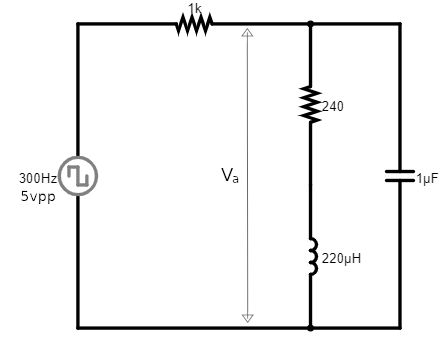
\includegraphics[width=5.5in]{images/diagram.PNG}
	\end{figure}
	\subsection*{Calculations}
	The calculations for this lab required us to determine the number of stages needed to meet the attenuation specifications of 70dB at 10KHz. We then calculated the values for the capacitors using scaling and choosing a resistor value of 1k $\Omega$.
	\subsubsection*{1. Approximate the number of stages needed to attain 70dB of attenuation.}
	Given:\\
	$f_{s}=10KHz$\\
	$f_{p}=1KHz$\\\\
	$n=\frac{-0.05A_{s}}{log(f_{s}/f_{p})}$\\
	$n=\frac{-0.05\cdot -70}{log(10KHz/1KHz)}=3.5$\\\\
	=>four stages should provide the required attenuation
	\subsubsection*{2. Using the roots from the Butterworth $n^{th}$ order polynomial table, calculate the roots of the polynomials for a fourth order filter.}
	Given:
	$(s^{2}+0.765s+1)(s^{2}+1.848s+1)$\\
	$C_{1}=2.61F$\\
	$C_{2}=0.38F$\\
	$C_{3}=1.08F$\\
	$C_{4}=0.924F$\\
	\subsubsection*{3. Using the values found above, scale the capacitors for the selected resistor value.}
	
	$R'=k_{m}R=1k\Omega$\\
	$k_{f}= \frac{\omega'_{c}}{\omega_{c}}=2000\pi$\\\\
	$C'=\frac{C}{k_{m}k_{f}}$\\
	$C'_{1}=\frac{C_{1}}{k_{m}k_{f}}=\frac{2.614F}{2000\pi\cdot1000}=416.0nF$\\
	$C'_{2}=\frac{C_{2}}{k_{m}k_{f}}=\frac{0.3825F}{2000\pi\cdot1000}=60.9nF$\\	
	$C'_{3}=\frac{C_{3}}{k_{m}k_{f}}=\frac{1.08F}{2000\pi\cdot1000}=171.9nF$\\ 
	$C'_{4}=\frac{C_{4}}{k_{m}k_{f}}=\frac{0.924F}{2000\pi\cdot1000}=147.1nF$\\ 
	\subsection*{Data Table}
		\begin{table}[H]
		\def\arraystretch{1.2}%
		\centering
		\begin{tabular}{|l|l|l|l|}
			\hline
			Frequency(Hz)		& $V_{out}$(ideal)		&  $V_{out}$(observed) 			&\% Diff	\\ \hline
			100  				& $10V$						& $10.05V$        			&0.5\%		\\ \hline	
			250					& $10.1V $					& $10.0V $    				&-0.99\%	\\ \hline
			500					& $10.3V$					& $9.6V$					&-6.80\%	\\ \hline
			600					& $10.3V$					& $9.25V$					&-10.19\%	\\ \hline
			700					& $10.2V$					& $8.75V$					&-14.22\%	\\ \hline
			800					& $9.6V$					& $8V$						&-16.67\%	\\ \hline
			900					& $8.5V$					& $7V$						&-17.65\%	\\ \hline
			1k					& $7V$						& $5.7V$					&-11.63\%	\\ \hline
			1.1k				& $5.4V$					& $4.6V$					&-8.0\%		\\ \hline
			1.2k				& $4V$						& $3.65V$					&-8.75\%	\\ \hline
			1.3k				& $3V$						& $2.8V$					&-6.67\%	\\ \hline
			1.5k				& $1.8V$					& $1.9V$					&5.56\%		\\ \hline
			2k					& $530mV$					& $700mV$					&32.07\%	\\ \hline
			3k					& $111mV$					& $200mV$					&80.2\%		\\ \hline
			4k					& $33mV$					& $75mV$					&127\%		\\ \hline
			5.5k				& $10mV$					& $32.5mV$					&225\%		\\ \hline				
	\end{tabular}
	\end{table}
	\subsection*{Procedure}
	The circuit was more involved than others we built in the class. We were able to successfully design the circuit based off of example 15.22 in the text in the first week of the lab. We also ran simulations of the lab in Orcad and met the calculations accordingly to ensure we would meet the design criteria. We then began building the circuit on a breadboard with the proper components in the second week, along with troubleshooting the circuit where necessary. Below is a picture of the circuit on the breadboard.
			
\begin{figure}[H]
	    \centering
	    \includegraphics[width=5.5in]{images/Circuit.jpg}
	 \end{figure}
	 \newpage
	\subsection*{Error Analysis}
	Our error analysis for this lab was good. Shown by the graph below our circuit preformed very closely with the simulated circuit and our average error in our data table from above was 35.7/%. 
	Our main sources of error were in the non-ideal components that were found in the lab. Also with the abundance of wires there was quite a bit of noise showing on the oscilloscope that we adjusted by adding another capacitor, shown on the left rail in the picture above. 			
	\begin{figure}[H]
		\centering
		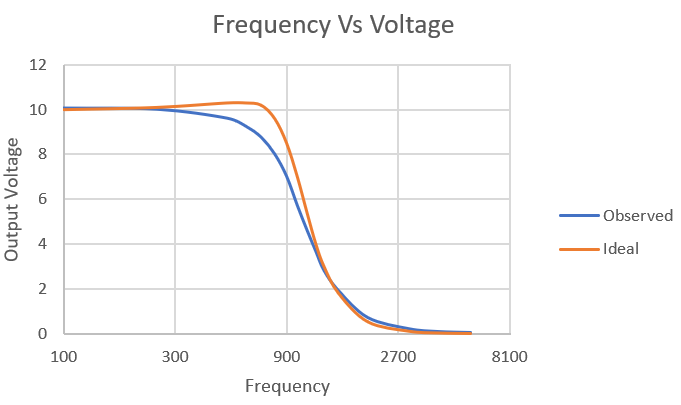
\includegraphics[width=5.5in]{images/comparison_graph.PNG}
	\end{figure}
\subsection*{Troubleshooting}
	We had several issues after initially building our circuit that we had to work through to get our circuit to function properly. Pins 2 and 3 on the Orcad Op Amp were switched and this error was carried through into building the circuit. Additionally, we had to add some capacitors to the output to buffer the waveform to achieve our desired voltage output. 
\subsection*{Conclusion}
	As stated above, this circuit design was more involved than previous labs. We designed, simulated, built and tested the chosen circuit within the two week requirement. We successfully calculated the nth order needed for the design and adjusted the passband by adding the 2Kohm resistor on the inverting amplifier. We achieved the minimum of -70db rolloff. We constructed, labeled, and simulated the diagram in Orcad, however we used HA17741 op amps rather than the suggested LM324. The Bode Plots with the ideal magnitude and phase are shown below. We tested our design on the oscilloscope successfully and took appropriate data.
\newpage
	\subsection*{Appendix A: Photos}
	\begin{figure}[H]
	\centering
		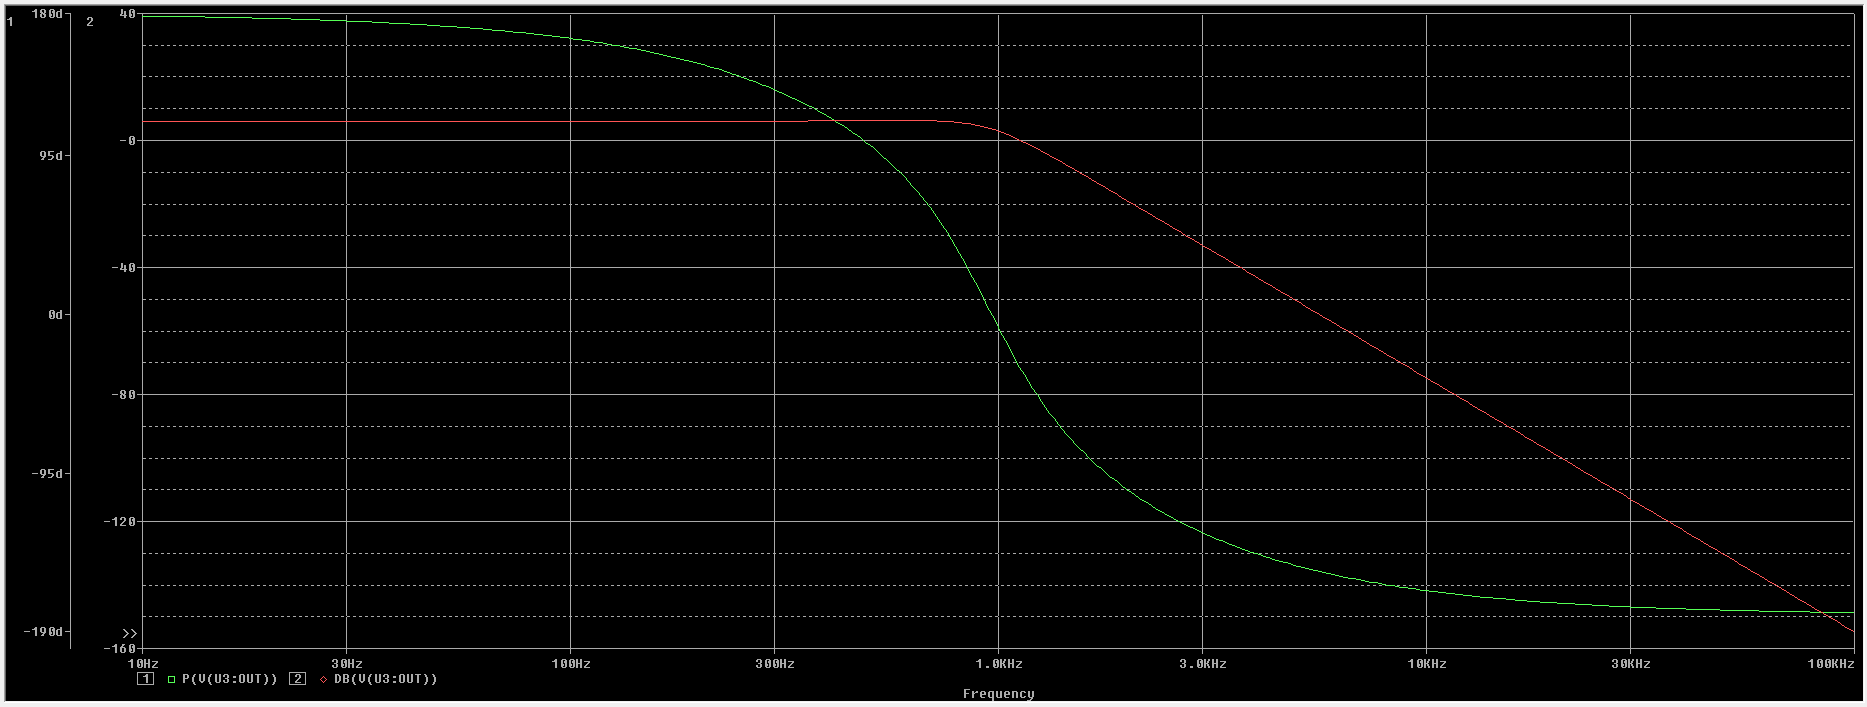
\includegraphics[width=5.5in]{images/Capture4 (phase info).png}
	\end{figure}
	\begin{figure}[H]
	\centering
		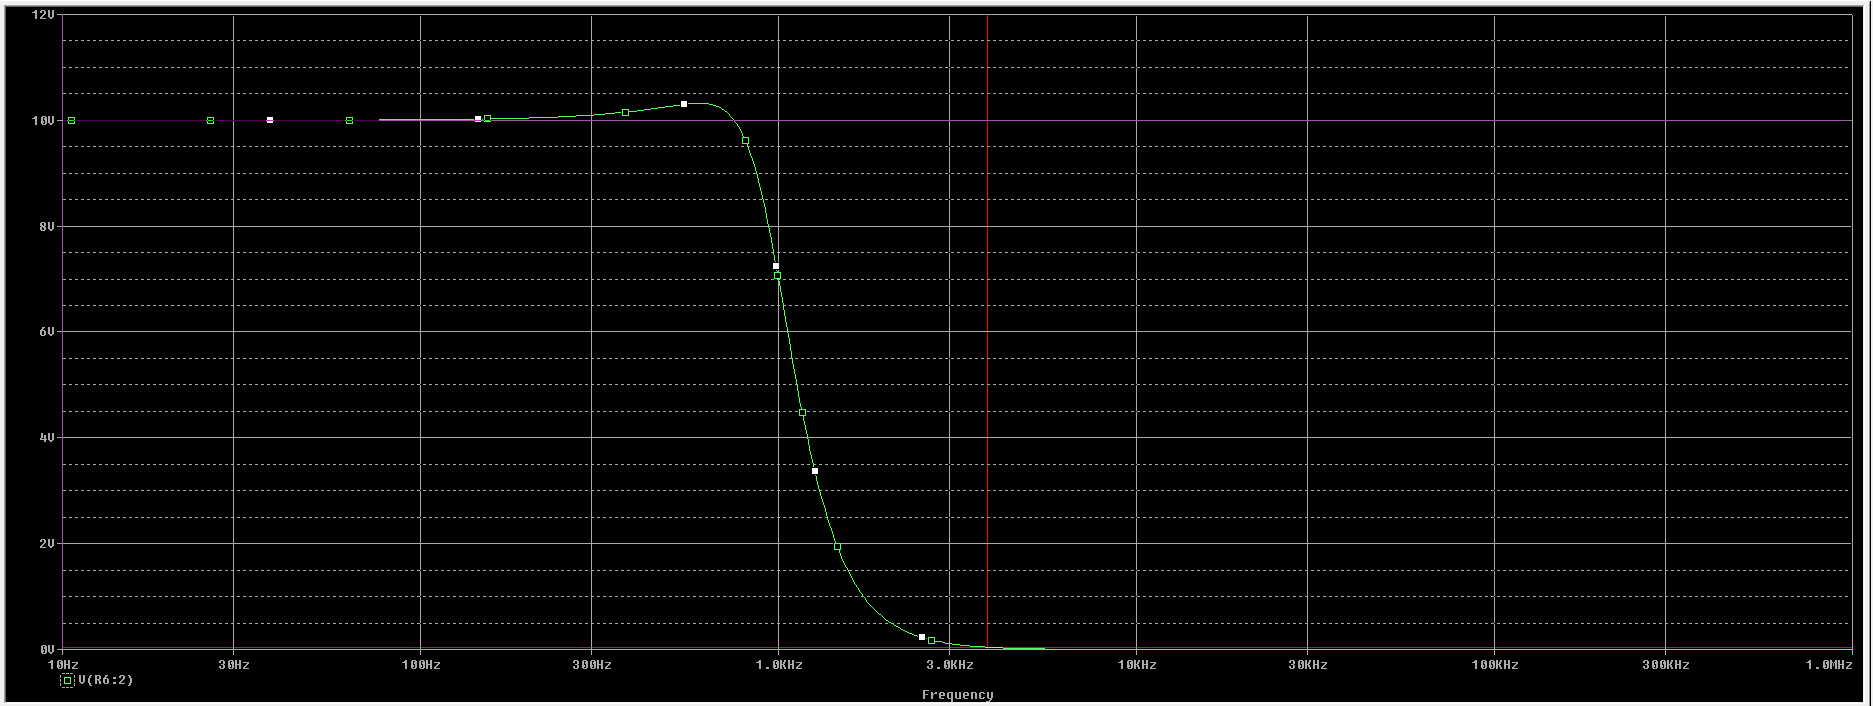
\includegraphics[width=5.5in]{images/CaptureWK2Graph.png}
	\end{figure}
\end{document}
